% !TeX spellcheck = en_US 
\documentclass[proposal]{byu-aero}

\newcommand{\nextyear}{2020}

%!!!!!!!!!!!!!!!!!!!!!!!!!!!!!!!!!!!!!!!!!!!!!!!!!!!!!!!!!!!!!!!!!!!!!!!!!!!!!!!!!!!!!!!!%
%!!!!!!! UNLESS YOU KNOW WHAT YOU'RE DOING, DO NOT TOUCH ANYTHING ABOVE THIS LINE !!!!!!!%
%!!!!!!!!!!!!!!!!!!!!!!!!!!!!!!!!!!!!!!!!!!!!!!!!!!!!!!!!!!!!!!!!!!!!!!!!!!!!!!!!!!!!!!!!%

%%%%%%%%%%%%%%%%%%%%%%%%%%%%%%%%%%
%%%%%%%%%%   Text Body   %%%%%%%%%
%%%%%%%%%%%%%%%%%%%%%%%%%%%%%%%%%%
\begin{document}

%%%%%%%%%%%%%%%%%%%%%%%%%%%%%%%%%%%%%%%%%%
%%%%%%%%%%   Executive Summary   %%%%%%%%%
%%%%%%%%%%%%%%%%%%%%%%%%%%%%%%%%%%%%%%%%%%
\section{Executive Summary (10 Points)}
\label{sec:ExecutiveSummary}

The key to the executive summary is to write it last (like an abstract). You should have the rest of the proposal done before starting on the Executive Summary.  In terms used by kids these days, the executive summary is the tl;dr version of the proposal. You should be able to gather \textit{all} of the important information from reading the executive summary, and it should be distilled down to concise terms. Generally, you should keep the executive summary to no more than a single page in length. Important things to include in the executive summary are:

\begin{itemize}
    \item Objective Statement
    \item Planned approach to achieve all objectives
    \item Main points from subsequent sections
\end{itemize}


%%%%%%%%%%%%%%%%%%%%%%%%%%%%%%%%%%%%%%%%%%%
%%%%%%%%%%   Management Summary   %%%%%%%%%
%%%%%%%%%%%%%%%%%%%%%%%%%%%%%%%%%%%%%%%%%%%
\section{Management Summary (40 Points)}
\label{sec:ManagementSummary}
%\begin{itemize}
%	\item Describe the organization, the roles of each team and individual skill sets required
%	\item Organization chart (by team/function, individual names are not required for the proposal)
%	\item Schedule / Major Milestone chart
%	\item Budget (not only for expected materials and manufacturing of the airplane, but for travel to the
%	competition site and any other expenses associated with the competition)
%\end{itemize}

You'll want to begin here with a paragraph describing the organization of the design team, citing \cref{fig:personnelassignments}. It's probably easiest to figure this out by diagramming it on a white board, and then creating a your flow chart in powerpoint, or something. You'll 

%TEAM ORGANIZATION
\begin{wrapfigure}[7]{R}{0in}
	\centering
	\raisebox{0pt}[\dimexpr\height-3\baselineskip\relax]{
\begin{tikzpicture}[node distance = 1cm, auto]

	% Place nodes
	\node [block] (Project Manager) {\footnotesize Project Manager};
%	\node [block, below left = 0.1 and -1.25cm  of Project Manager] (Engineering Lead) {\footnotesize Engineering Lead};
%	\node [block, below right = 0.1 and -1.25cm   of Project Manager] (Project Manager) {\footnotesize Project Manager};

	\node [block2, below left = 0.25 and -1.25cm of Project Manager] (Aerodynamics) {\footnotesize Aerodynamics};
	\node [block2, below left = 1.0 and -1.25cm  of Project Manager] (Structures) {\footnotesize Structures};
	\node [block2, below left = 1.75 and -1.25cm  of Project Manager] (Propulsion) {\footnotesize Propulsion};
	\node [block2, below right = 0.25 and -1.25cm  of Project Manager] (Systems) {\footnotesize Systems};
	\node [block2, below right = 1.0 and -1.25cm  of Project Manager] (Graphics) {\footnotesize Graphics};
	\node [block2, below right = 1.75 and -1.25cm  of Project Manager] (Manufacturing) {\footnotesize Manufacturing};

	% Draw edges
%	\path[line] let \p1=(Project Manager.south), \p2=(Engineering Lead.east) in (Project Manager.south) --  +(0,0.55*\y2) -| node {} (Engineering Lead.east);
%	\path[line] let \p1=(Project Manager.south), \p2=(Project Manager.west) in (Project Manager.south) -- +(0,0.55*\y2) -| node {} (Project Manager.west);

	\path[line] let \p1=(Project Manager.south), \p2=(Aerodynamics.east) in (Project Manager.south) -- +(0,0.65*\y2) -| node  {} (Aerodynamics.east);
	\path[line] let \p1=(Project Manager.south), \p2=(Systems.west) in (Project Manager.south) -- +(0,0.65*\y2) -| node  {} (Systems.west);

	\path[line] let \p1=(Project Manager.south), \p2=(Structures.east) in (Project Manager.south) -- +(0,0.8*\y2) -| node  {} (Structures.east);
	\path[line] let \p1=(Project Manager.south), \p2=(Graphics.west) in (Project Manager.south) -- +(0,0.8*\y2) -| node  {} (Graphics.west);

	\path[line] let \p1=(Project Manager.south), \p2=(Propulsion.east) in (Project Manager.south) -- +(0,0.85*\y2) -| node  {} (Propulsion.east);
	\path[line] let \p1=(Project Manager.south), \p2=(Manufacturing.west) in (Project Manager.south) -- +(0,0.85*\y2) -| node  {} (Manufacturing.west);
\end{tikzpicture}}
	\caption{Here we show the structure of, and assignment areas within, our team organization.}
	\label{fig:personnelassignments}
\end{wrapfigure}

\Cref{fig:plannedtiming} shows our planned project schedule. We have subdivided the project into four phases, each lasting six weeks %Wrapped Figure Example. [#of lines the figure is long]{where (capitalization matters)}{how much it is moved}
\begin{wrapfigure}[6]{r}{5cm}
	
\includegraphics[width=1.5in]{draft.pdf}
	\caption{Example of Wrapped figure}
	\label{fig:wrappedfig}
\end{wrapfigure} (with an additional 5 week buffer for the final manufacturing of our design). Since the conceptual design is a major deliverable for this proposal, we have already completed this phase, and have moved on to Phase II: Preliminary Design. For the sake of brevity of this proposal, we will forgo including the beginnings of our preliminary design, and report its entirety in the final design report.

% expanded CO architecture diagram produced by the TikZ package
\documentclass[]{byu-aero}

\def \theyear {2020}
\def \nextyear {2021}

\usepackage[active,tightpage]{preview}
\PreviewEnvironment{tikzpicture}
\setlength{\PreviewBorder}{0em}


%GANTT CHART
\usepackage{pgfgantt}
\ganttset{
	time slot format=isodate,
	time slot unit=day,
	x unit=0.025cm,
	y unit title=0.4cm,
	y unit chart=0.3cm,
	hgrid,
	canvas/.append style={draw=\BYUblue},
	%
	title label font=\bfseries\scriptsize,
	title height=1,
	title/.style={fill=\BYUbluelite,draw=\BYUblue},
	%
	today = \theyear-10-30,
	today label = Current Date,
	today label font=\itshape\tiny,
	today rule/.style={draw=\BYUgray,dashed},
	%
	group/.append style={fill=\BYUbluemid,draw=\BYUblue},
	group top shift=0.25,
	group height=.25,
	group right peak tip position=0.0,
	group left peak tip position=0.0,
	group peaks width=2.0,
	group peaks height=0.25,
	group label font = \bfseries\footnotesize,
	%
	bar/.append style={fill=\BYUblue,draw=\BYUblue},
	bar label font=\footnotesize,
	bar height = 0.25,
	%	bar top shift = 0.25,
	progress label text = {},
	%
	milestone/.append style={fill=\BYUbluelite,draw=\BYUblue,xscale=12},
	milestone height = 0.95,
	milestone top shift = 0.0,
	milestone label font = \itshape\footnotesize,
	%
	%	link/.append style={draw=\BYUblue},
	link tolerance = 10,
	link bulge = 10,
}


\begin{document}
	\begin{figure}[h!]
		\centering
		\begin{ganttchart}[]{\theyear-09-01}{\nextyear-04-30}
			\gantttitlecalendar{year, month=shortname} \\
			%
			%%--DESIGN--%%
			%
			\ganttgroup{Design}{\theyear-09-14}{\nextyear-01-28} \\
			\ganttbar[progress=100]{Conceptual Design}{\theyear-09-14}{\theyear-10-07} \\
			\ganttbar[progress=0]{Preliminary Design}{\theyear-10-31}{\theyear-12-01} \\
			\ganttbar[progress=0]{Detailed Design}{\theyear-12-28}{\nextyear-01-28} \\
			%
			%%--PROTOTYPING--%%
			%
			\ganttgroup{Build}{\theyear-10-01}{\nextyear-02-01} \\
			\ganttbar[progress=100]{Conceptual Prototypes}{\theyear-10-01}{\theyear-10-14} \\
			\ganttbar[progress=0]{Preliminary Prototypes}{\theyear-11-14}{\theyear-12-14} \\
			\ganttbar[progress=0]{Detailed Prototypes}{\nextyear-01-07}{\nextyear-02-01} \\
			\ganttbar[progress=0]{Final Build}{\nextyear-02-20}{\nextyear-03-21}\\
			%
			%%--TESTING--%%
			%
			\ganttgroup{Fly}{\theyear-10-07}{\nextyear-03-28} \\
			\ganttbar[progress=100]{Conceptual Testing}{\theyear-10-07}{\theyear-10-28}\\
			\ganttbar[progress=0]{Preliminary Testing}{\theyear-12-01}{\theyear-12-21}\\
			\ganttbar[progress=0]{Detailed Testing}{\nextyear-01-14}{\nextyear-02-07}\\
			\ganttbar[progress=0]{Practice Runs}{\nextyear-03-21}{\nextyear-03-28}\\
			%
			%%--COMPETING--%%
			%
			\ganttgroup{Competition Milestones}{\theyear-10-30}{\nextyear-04-16} \\
			\ganttmilestone{Submit Proposal}{\theyear-10-30} \\
			\ganttmilestone{Preliminary Design Review}{\theyear-12-21} \\
			\ganttmilestone{Submit Design Report}{\nextyear-02-20} \\
			\ganttmilestone{Submit Proof of Flight}{\nextyear-04-01} \\
			\ganttmilestone{Fly-off}{\nextyear-04-16}
			%
			%
			%%--VERTICAL RULE--%%
%			\ganttvrule[vrule/.append style={draw=\BYUgray}]{\tiny \textit{Current Date}}{\theyear-10-30}
			today=\theyear-10-30
			%
			%%--LINKS--%%
			%
			\ganttlink[link/.append style={draw=\BYUblue}]{elem1}{elem5}
			\ganttlink[link/.append style={draw=\BYUblue}]{elem5}{elem10}
			\ganttlink[link/.append style={draw=\BYUblue}]{elem10}{elem15}
			%
			\ganttlink[link/.append style={draw=\BYUred}]{elem2}{elem6}
			\ganttlink[link/.append style={draw=\BYUred}]{elem6}{elem11}
			\ganttlink[link/.append style={draw=\BYUred}]{elem11}{elem16}
			%
			\ganttlink[link/.append style={draw=\BYUgreen}]{elem3}{elem7}
			\ganttlink[link/.append style={draw=\BYUgreen}]{elem7}{elem12}
			\ganttlink[link/.append style={draw=\BYUgreen}]{elem12}{elem17}
		\end{ganttchart}
	\end{figure}
	
\end{document}

\subsection{Budget}
\label{ssec:budget}

Put together a budget. Not much to it.

Here is an example of a wrapped table just in case you need more room. Note that the wrapped figures and tables need to be sandwiched between text in order to work.  Also note that if you don't have a lot of text, 
% Project Budget
\begin{wraptable}[]{r}{5cm}
	\centering
	\renewcommand*{\arraystretch}{1.2}
	\caption{Project Budget}
	\label{tab:budget}
	\rowcolors{2}{BYUbluelite}{white}
	\begin{tabular}{ |c|c| } 
		\hline
		\rowcolor{BYUbluemid}
		Item & Cost (\$) \\ 
		\hline
		&  \\ 
		&  \\ 
		&  \\ 
		&  \\ 
		\hline
		\textbf{Total} & \textbf{} \\ 
		\hline
		
	\end{tabular}
\end{wraptable}
weird spacing occurs. Wrapped tables and figures also just do weird stuff in general (like not staying withing the text bounds of the page and making weird white spaces where you don't want them.) In general, they should be avoided, especially for important things.


%%%%%%%%%%%%%%%%%%%%%%%%%%%%%%%%%%%%%%%%%%
%%%%%%%%%%   Conceptual Design   %%%%%%%%%
%%%%%%%%%%%%%%%%%%%%%%%%%%%%%%%%%%%%%%%%%%
\section{Conceptual Design Approach (20 Points)}
\label{sec:ConceptualDesign}
%\begin{itemize}
%    \item Decomposition of mission requirements into sub-system requirements.
%    \item Preliminary design / sizing results; concept sketch, if available (does not have to be representative of the final design) 
%    \item Sensitivity Study of Design Parameters
%\end{itemize}

\subsection{Mission Requirements}
\label{ssec:missionreqs}

Decomposition of mission requirements into sub-system requirements.

\subsubsection{Aerodynamic Requirements}
\label{sssec:aeroreqs}

\subsubsection{Structural Requirements}
\label{sssec:structreqs}

\subsubsection{Propulsion Requirements}
\label{sssec:propreqs}

\subsubsection{Specialty Requirements} %change this to be specifically what it is (like bomb drop or whatever the specific mission is)
\label{sssec:specialreqs}

\subsection{Preliminary Design}
\label{ssec:preliminarydesign}

Preliminary design / sizing results; concept sketch, if available (does not have to be representative of the final design) 


%\begin{figure}[h!]
%	\centering
%	\begin{subfigure}[t]{0.475\textwidth} % width of left subfigure
%		\centering
%		
\includegraphics[width=\textwidth]{draft.pdf}
%		\caption{The left side image}
%		\label{fig:a}
%	\end{subfigure}
%	\hfill
%	\begin{subfigure}[t]{0.475\textwidth} % width of right subfigure
%		\centering
%		
\includegraphics[width=\textwidth]{draft.pdf}
%		\caption{The rigth side image}
%		\label{fig:b}
%	\end{subfigure}
%	\caption{This is an example of a subfigure figure.}
%	\label{fig:subex}
%\end{figure}

% Concept Sketch
\begin{figure}[h!]
	\centering
	
\includegraphics[width=3.5in]{draft.pdf}
	\caption{Here we show a concept sketch of our current design iteration.}
	\label{fig:conceptsketch}
\end{figure}

\subsection{Sensitivity Studies}
\label{ssec:sensitivitystudies}

Sensitivity Study of Design Parameters

%%%%%%%%%%%%%%%%%%%%%%%%%%%%%%%%%%%%%%%%%%%
%%%%%%%%%%   Manufacturing Plan   %%%%%%%%%
%%%%%%%%%%%%%%%%%%%%%%%%%%%%%%%%%%%%%%%%%%%
\section{Manufacturing Plan (15 Points)}
\label{sec:ManufacturingPlan}
\begin{itemize}
    \item Preliminary manufacturing flow
    \item Describe critical processes or technologies required
\end{itemize}

% Manufacturing Flow Chart
\begin{figure}[h!]
	\centering
	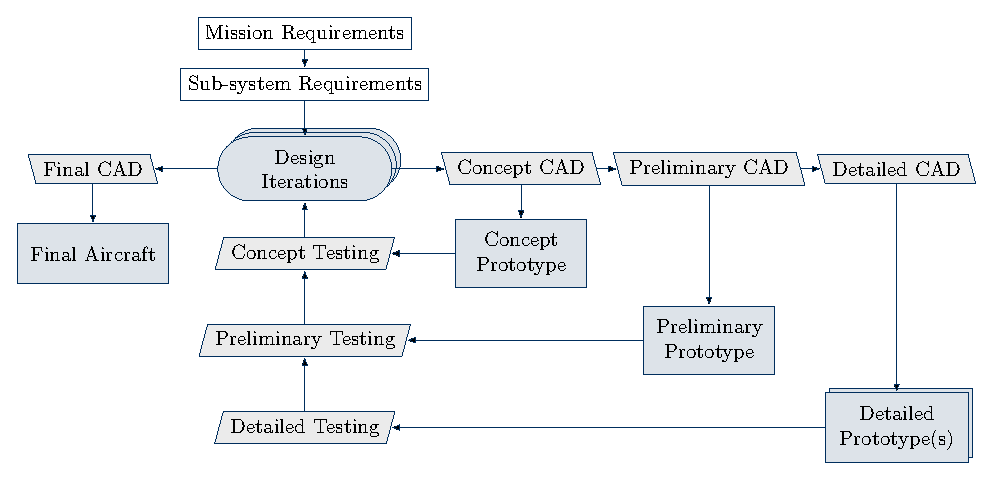
\includegraphics[width=4.5in]{manufacturing_flow.pdf}
	\caption{We show here an extended design structure matrix of our proposed manufacturing plan.}
	\label{fig:manufacturingplan}
\end{figure}


%%%%%%%%%%%%%%%%%%%%%%%%%%%%%%%%%%%%%
%%%%%%%%%%   Testing Plan   %%%%%%%%%
%%%%%%%%%%%%%%%%%%%%%%%%%%%%%%%%%%%%%
\section{Testing Plan (15 points)}
\label{sec:TestingPlan}
\begin{itemize}
    \item Component and ground test plan
    \item Flight test plan 
\end{itemize}


%%%%%%%%%%%%%%%%%%%%%%%%%%%%%%%%%%%%%
%%%%%%%%%%   Bibliography   %%%%%%%%%
%%%%%%%%%%%%%%%%%%%%%%%%%%%%%%%%%%%%%
%Bibliography (5 Points)
%\item List of all published works referenced in the text must be present in this section.
%\item Any material taken from a published source in all previous sections must have a numerical subscript corresponding to the appropriate citation in this section.
%\item References should appear in numerical order.
%\item Format should match AIAA provided guidelines:
%\newpage
%\clearpage
%\bibliography{ref}{}
%\bibliographystyle{aiaa}

\end{document}